\documentclass[fontsize=12pt, paper=a4]{scrartcl}

\usepackage{fontspec}
\usepackage{graphicx}
\usepackage{booktabs}


\begin{document}


\begin{table}
\caption{My fancy summary table}
\begin{tabular}{lll}
\input{t_census.tex}
\end{tabular}
\end{table}

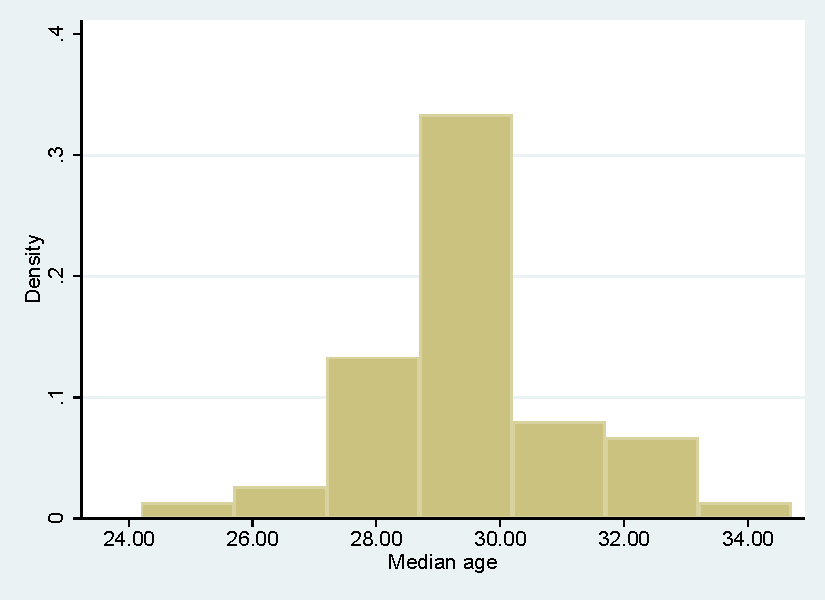
\includegraphics[width=\textwidth]{hist-plot-age}


%% https://tex.stackexchange.com/questions/50694/cannot-use-toprule-when-doing-input-inside-tabular-why
\begin{table}[h]
\caption{Another fancy summary table}
\begin{tabular}{rrrrrrrr}
%% WICHTIG: \toprule muss ausserhalb der via \input eingebundenen Tabelle stehen!
\toprule
\input{t_write-file-sample.tex}
%% DOES NOT WORK: \bottomrule
\end{tabular}
\end{table}


\end{document}